\begin{figure*}[t]
\centering
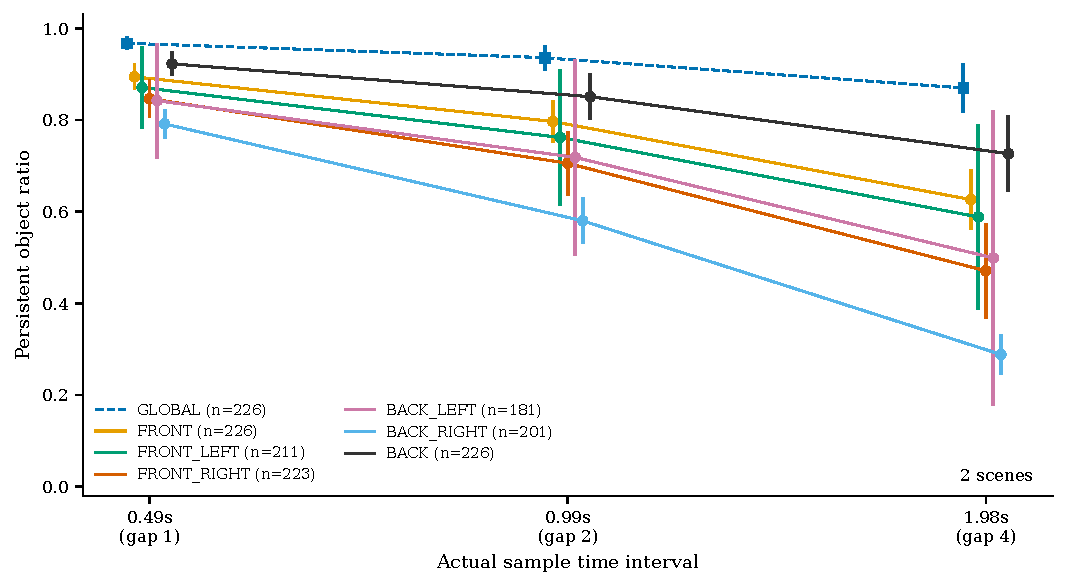
\includegraphics[width=0.95\textwidth]{figure_pdf/M2a_physical_persistence.pdf}
\caption{Global annotated persistence and camera projected-in-view persistence use separate sets and different denominators; the curve gap is not a decomposition. Scene-equal pair means; 95\% scene-bootstrap intervals; n counts pairs with a nonempty initial set, summed over gaps in each legend. Actual mean sample gaps are shown; camera exposure gaps are recorded separately.}
\label{fig:M2a_physical_persistence}
\end{figure*}

\begin{figure*}[t]
\centering
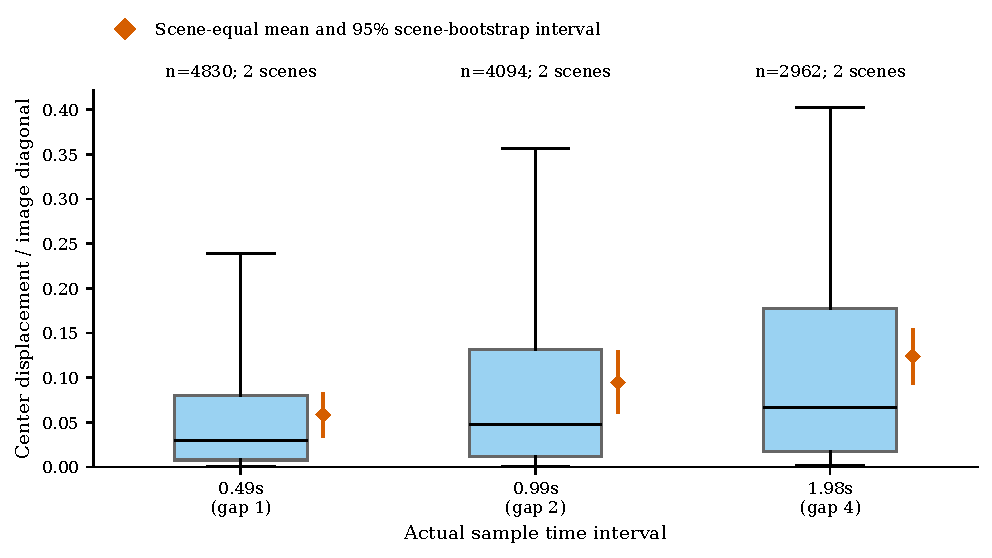
\includegraphics[width=0.95\textwidth]{figure_pdf/M2b_image_displacement.pdf}
\caption{Same official instance ID, same camera and scene, valid projections at both times. Boxes: pooled 25–75\%, median; whiskers: 5–95\%. Orange diamonds: scene-equal means with 95\% scene-bootstrap intervals. n is camera-pair instance observations; repeated temporal pairs, repeated instances and cross-camera projections are dependent.}
\label{fig:M2b_image_displacement}
\end{figure*}

\begin{figure*}[t]
\centering
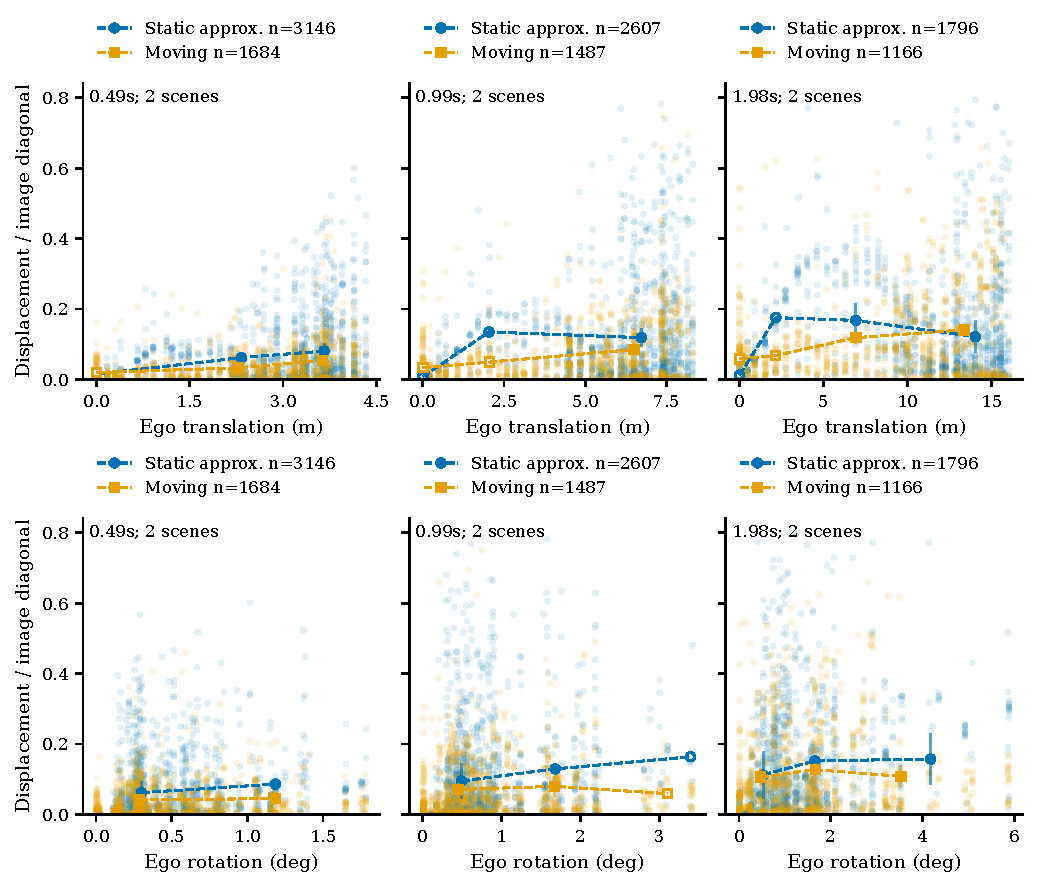
\includegraphics[width=0.95\textwidth]{figure_pdf/M2c_ego_motion_displacement.pdf}
\caption{Time-gap strata; approximately static means global annotation-center speed ≤0.5 m/s over actual sample timestamps. Scatter is seeded and independently capped at 1,200 observations per group, so it does not encode group frequency; binned summaries use all rows. X medians count each unique camera pair once; y is scene-equal displacement mean with 95\% scene-bootstrap intervals. Open markers denote one-scene bins without CIs; exact per-bin observation and scene counts are in metadata/figure\_bin\_counts.json. Dashed segments connect bin summaries, not a fitted causal response. Associations do not establish ego-only causation.}
\label{fig:M2c_ego_motion_displacement}
\end{figure*}

\begin{figure*}[t]
\centering
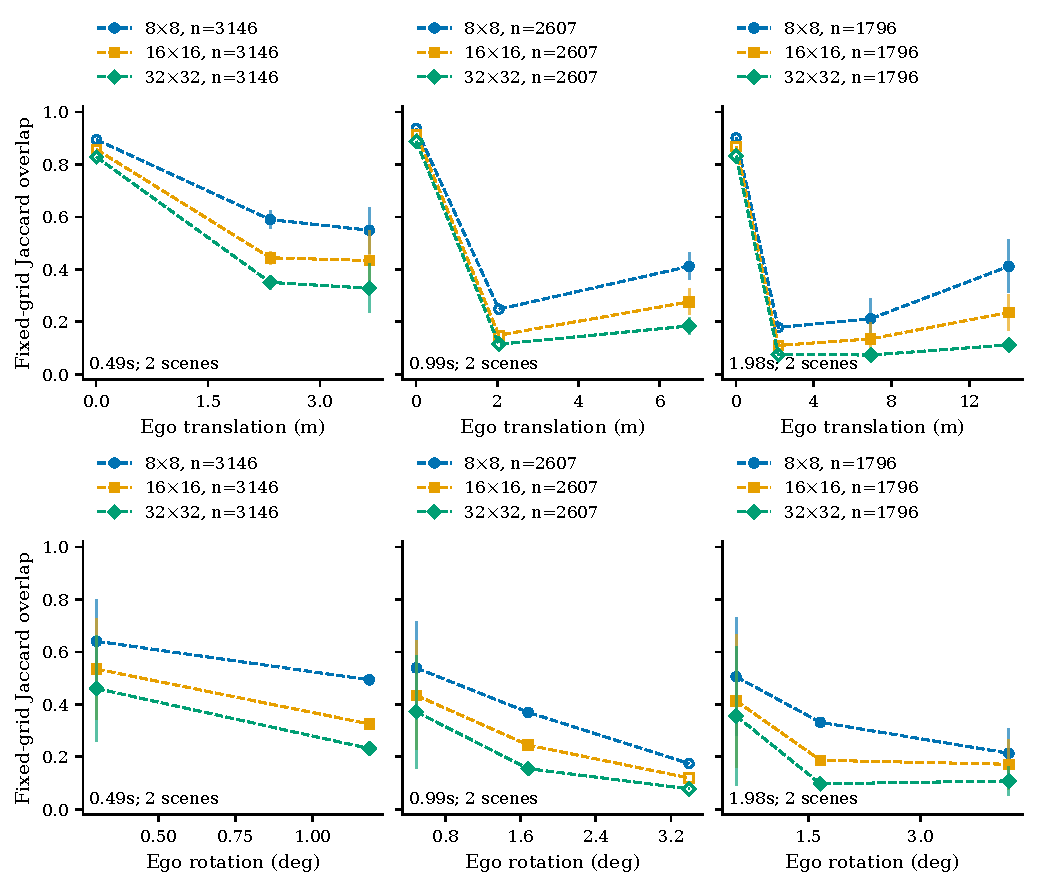
\includegraphics[width=0.95\textwidth]{figure_pdf/M2d_grid_overlap.pdf}
\caption{Approximately static annotated objects only: global annotation-center speed ≤0.5 m/s over actual sample timestamps. Main rule any: positive-area box/cell intersection. Grids are diagnostic image regions, not CLIP tokens. X medians count unique camera pairs once; y is scene-equal Jaccard mean with 95\% scene-bootstrap intervals. Open markers denote singleton-scene bins without CIs; exact per-bin counts are in metadata/figure\_bin\_counts.json. Grid variants share the same underlying observations and are not independent objects. Dashed segments connect bin summaries.}
\label{fig:M2d_grid_overlap}
\end{figure*}

\begin{figure*}[t]
\centering
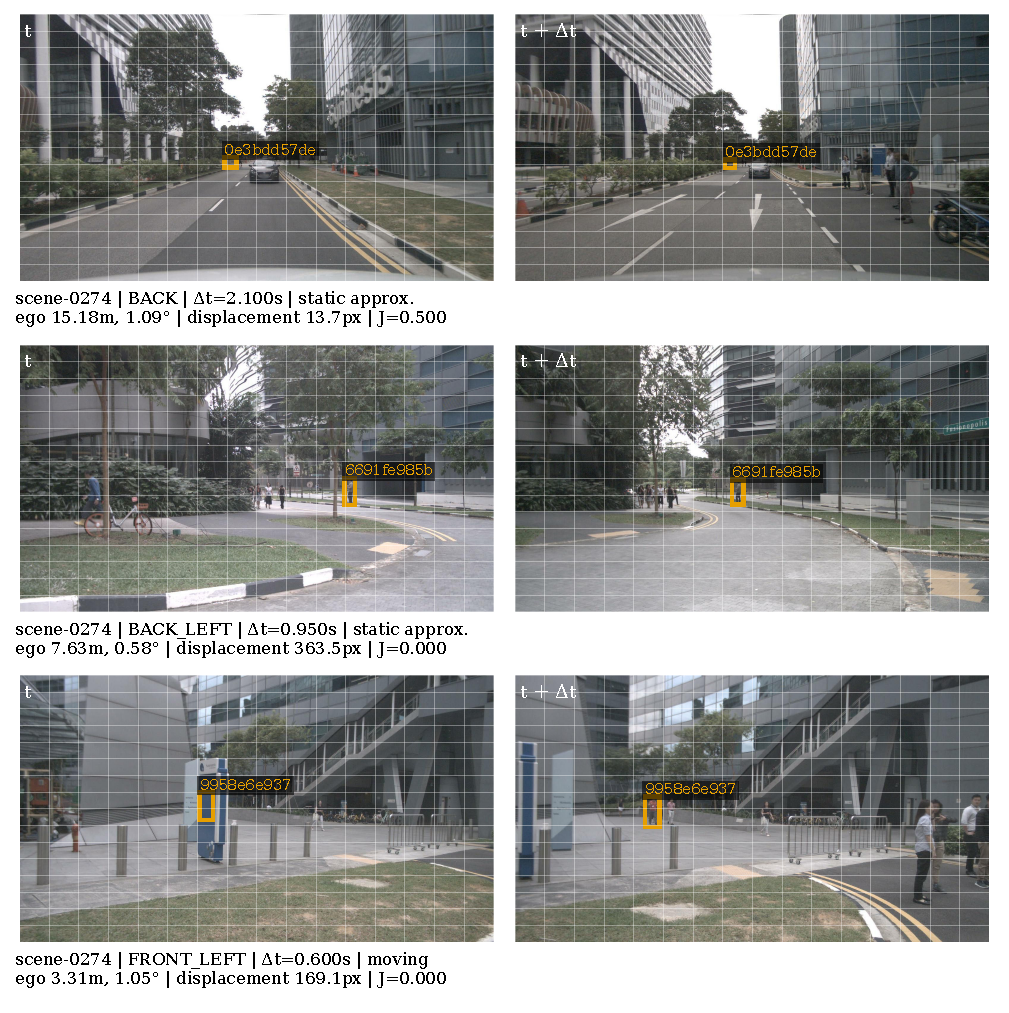
\includegraphics[width=0.95\textwidth]{figure_pdf/M2e_qualitative_examples.pdf}
\caption{The two gold rectangles within each row mark the matched official instance; labels show ten-character token prefixes (full IDs in metadata/CSV). Fixed [16, 16] grid, any overlap. Seeded scene/camera/gap/motion round-robin strata with 5–95\% quantile targets include both small and large displacement; cases are illustrative, not statistical evidence. Page 1/2; 6 individual examples saved.}
\label{fig:M2e_qualitative_examples}
\end{figure*}

\begin{figure*}[t]
\centering
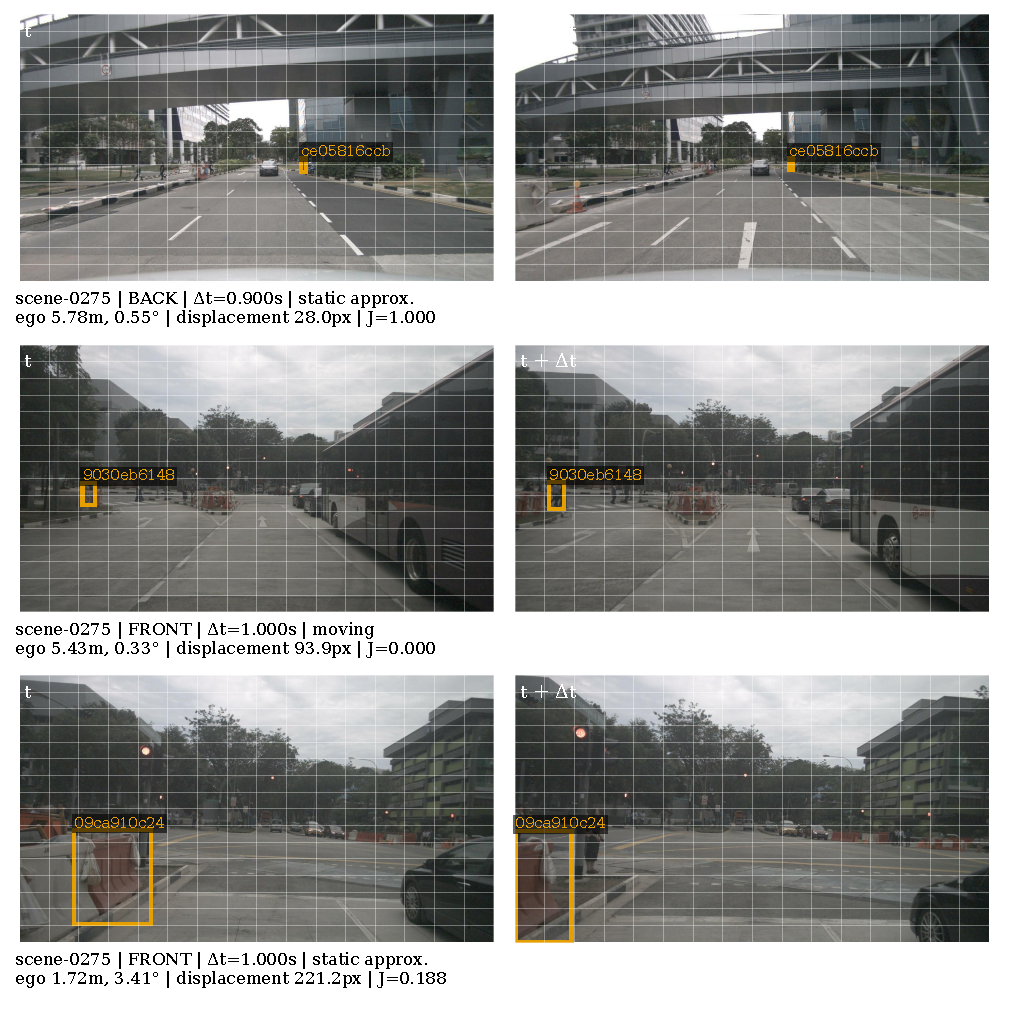
\includegraphics[width=0.95\textwidth]{figure_pdf/M2e_qualitative_examples_page2.pdf}
\caption{The two gold rectangles within each row mark the matched official instance; labels show ten-character token prefixes (full IDs in metadata/CSV). Fixed [16, 16] grid, any overlap. Seeded scene/camera/gap/motion round-robin strata with 5–95\% quantile targets include both small and large displacement; cases are illustrative, not statistical evidence. Page 2/2; 6 individual examples saved.}
\label{fig:M2e_qualitative_examples_page2}
\end{figure*}
